\documentclass{article}[18pt]
\usepackage[utf8]{inputenc}
\usepackage[margin=0.7in]{geometry}
\usepackage{parselines} 
\usepackage{amsmath}
\usepackage{titlesec}
\usepackage{pgfplots}
\usepackage{graphicx}
\usepackage[english]{babel}
\usepackage{fancyhdr}
\usepackage{tikz}
\usetikzlibrary{scopes}
\pgfplotsset{width=10cm,compat=1.9}
\usepackage{gensymb}

\titlespacing\section{0pt}{14pt plus 4pt minus 2pt}{0pt plus 2pt minus 2pt}
\newlength\tindent
\setlength{\tindent}{\parindent}
\setlength{\parindent}{0pt}
\renewcommand{\indent}{\hspace*{\tindent}}

\pagestyle{fancy}
\fancyhf{}
\rhead{Sam Robbins 13SE}
\lhead{A Level Physics - Further Mechanics and Thermal Physics}
\rfoot{Page \thepage}
\pgfdeclarelayer{background layer}
\pgfdeclarelayer{foreground layer}
\pgfsetlayers{background layer,main,foreground layer}

\begin{document}
\begin{center}
\underline{\huge Thermal Physics}
\end{center}
\section{Differences between heat and temperature}
\begin{tabular}{|c|c|c|}
\hline
&Heat&Temperature\\
\hline
Definition&Thermal energy(transferred from hot to cooler places)&A comparative measure of how hot something is\\
\hline
Unit&Joule&Kelvin\\
\hline
Measured using&Joulemeter&Thermometer\\
\hline
\end{tabular}
\section{Graph of heating water}
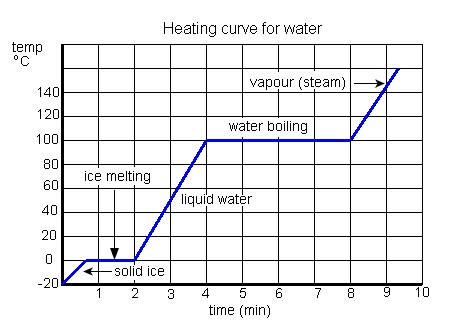
\includegraphics[width=3in]{water_heat_curve.jpg}
\section{Specific heat capacity}
\textbf{Specific heat capacity} - The energy needed to raise the temperature of 1kg of a material by 1K\\
\\
$c=\dfrac{Q}{m\Delta\theta}$\\
\\
c=Specific heat capacity - $Jkg^{-1} \ \degree C$\\
m=Mass - $kg$\\
$\Delta\theta$ = Temperature change - $\degree C$\\
Q = Heat energy - $J$
\subsection{Latent heat}
\textbf{Specific latent heat of fusion, $\mathbf{L_f}$} \quad \textcolor{red}{$Q=mL_f$}\\
The energy needed to change 1kg of a solid to a liquid without a temperature change\\
\\
\textbf{Specific latent heat of vaporisation, $\mathbf{L_v}$} \quad \textcolor{red}{$Q=mL_v$}\\
The energy needed to change 1kg of a liquid to a vapour without a temperature change

\end{document}